\section{8.7. Training}

% SLIDE CHUYỂN PHẦN 8.7
\begin{frame}{Nội dung trình bày}
	\tableofcontents[currentsection]
\end{frame}

% SLIDE 12
\begin{frame}{8.7. Hàm mục tiêu Cross-Entropy}
	
	\textbf{Cơ sở Đánh giá (Loss Function):}
	\begin{itemize}
		\item Các mô hình ngôn ngữ lớn (LLM) được huấn luyện bằng \textbf{hàm mất mát Cross-Entropy}, hay còn gọi là \textbf{Negative Log-Likelihood}.
		\item Tại bước thời gian $t$, mức phạt là \textbf{logarit âm của xác suất} dự đoán từ đúng:
	\end{itemize}
	
	$$L_t = -\log p(w_{t+1})$$
	
	\vspace{0.3cm}
	
	\textbf{Tối ưu hóa Trọng số:}
	\begin{itemize}
		\item Mất mát của chuỗi là \textbf{trung bình cộng Cross-Entropy} trên toàn bộ chuỗi có độ dài $T$:
	\end{itemize}
	
	$$L = -\frac{1}{T} \sum_{t=1}^{T} \log p(w_{t})$$
	
	\begin{itemize}
		\item Trọng số mạng nơ-ron được \textbf{cập nhật qua Gradient Descent} nhằm \textbf{tối thiểu hóa Loss trung bình} này.
	\end{itemize}
	
\end{frame}

% SLIDE 13
\begin{frame}{8.7. Khả năng Huấn luyện Song song}
	\begin{columns}
		\begin{column}{0.5\textwidth}
			\textbf{Xử lý song song (Parallelism):}
			\begin{itemize}
				\item Đầu ra cho mỗi phần tử trong chuỗi được \textbf{tính toán một cách độc lập}.
				\item Nhờ cấu trúc này, mỗi phần tử huấn luyện có thể được \textbf{xử lý song song}.
				\item Quá trình này \textbf{khắc phục hoàn toàn điểm yếu tính toán} của các mạng \textbf{RNN truyền thống}.
			\end{itemize}
		\end{column}
		\begin{column}{0.5\textwidth}
			\centering
			% Hình tài liệu cung cấp
			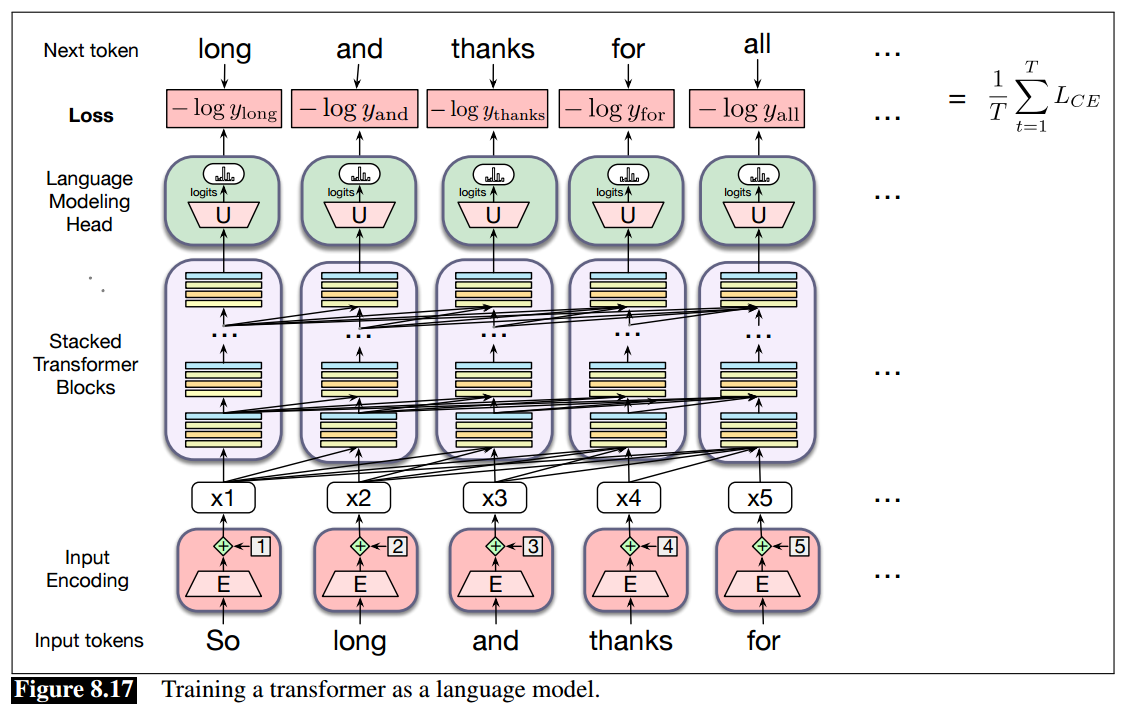
\includegraphics[width=1\textwidth, height=0.7\textheight, keepaspectratio]{img/figure8_17.png}
		\end{column}
	\end{columns}
\end{frame}

% SLIDE 14
\begin{frame}{8.7. Quản lý Quy mô Dữ liệu (Data Scaling)}
	
	\textbf{Kỹ thuật tối ưu hóa phần cứng:}
	
	\vspace{0.4cm}
	
	\begin{itemize}
		\setlength{\itemsep}{0.4cm} % Tăng khoảng cách giữa các mục để slide bớt trống
		\item \textbf{Cửa sổ ngữ cảnh:} Các mô hình lớn được huấn luyện bằng cách lấp đầy toàn bộ cửa sổ ngữ cảnh (ví dụ: 4096 tokens cho GPT-4, 8192 cho Llama 3).
		\item \textbf{Data Packing:} Nếu tài liệu gốc ngắn hơn cửa sổ, nhiều tài liệu sẽ được "đóng gói"\ chung và ngăn cách bởi một token \textit{\textbf{end-of-text}} đặc biệt.
		\item \textbf{Batch Size:} Kích thước lô dùng cho Gradient Descent thường rất lớn.
	\end{itemize}
	
\end{frame}
